\section{Résultats et évaluation du pipeline}
\begin{frame}
    \frametitle{Résultats: effet des itérations et du batch}
    \begin{columns}[T,totalwidth=\textwidth]
        \column{0.5\textwidth}
        \centering
        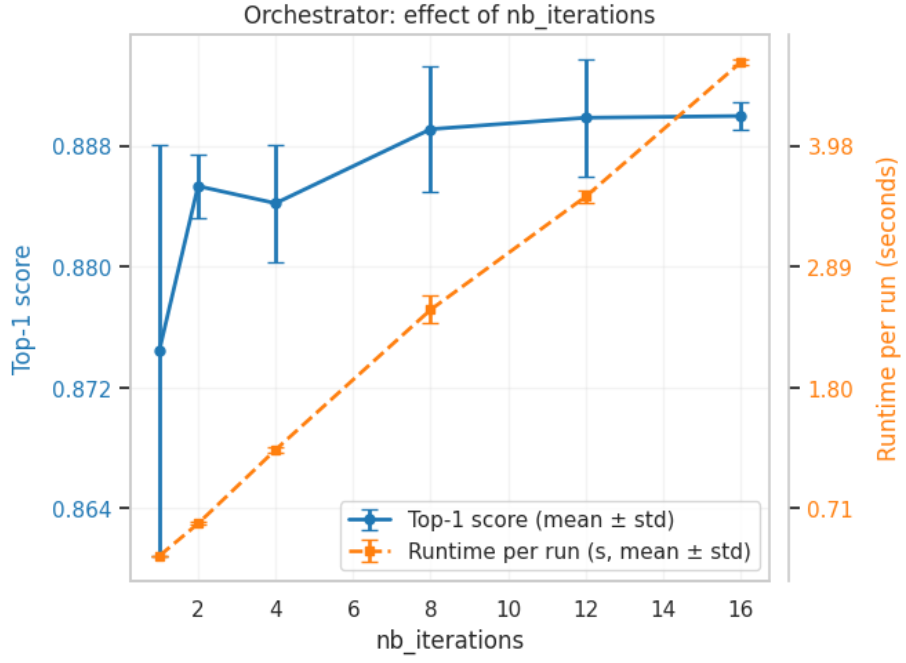
\includegraphics[width=\linewidth]{images/pipeline_effect_of_nb_iterations.png}

        \column{0.5\textwidth}
        \centering
        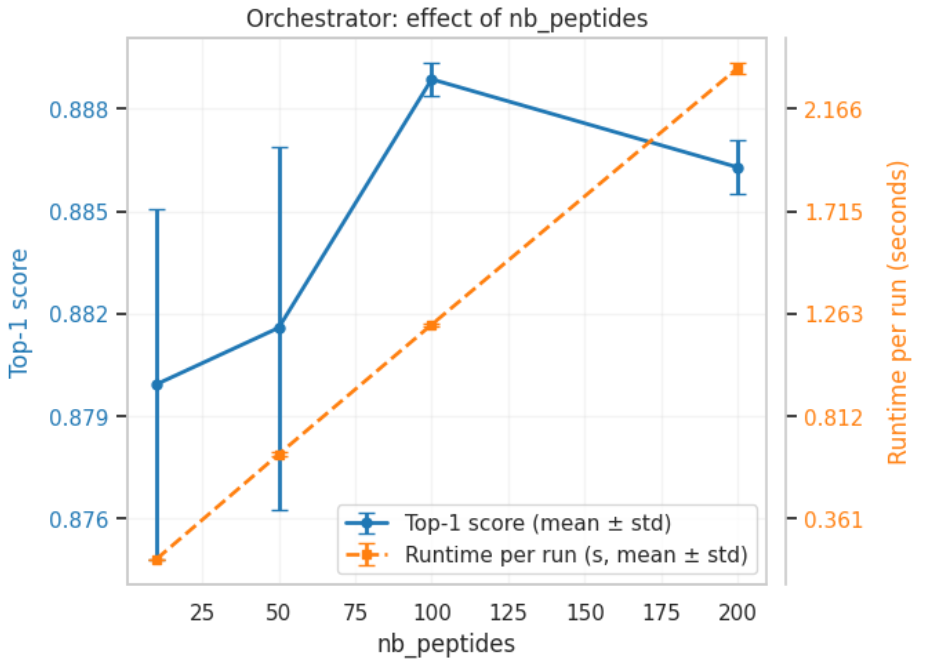
\includegraphics[width=\linewidth]{images/pipeline_effect_of_nb_peptide.png}
    \end{columns}
    \raggedleft \tiny \textcolor{gray}{Runtime: RTX 4070 (Portable), Ryzen 7350XT, 16Go RAM}

    \begin{block}{Analyse}
        \scriptsize
        Augmenter le budget de recherche améliore très légèrement la qualité mais rapidement le runtime, suggérant une possibilitée d'amélioration d'orchestrateur.
    \end{block}
\end{frame}

\begin{frame}
    \frametitle{Résultats: impact de la longueur cible}
    \begin{columns}[T,totalwidth=\textwidth]
        \column{0.60\textwidth}
        \centering
        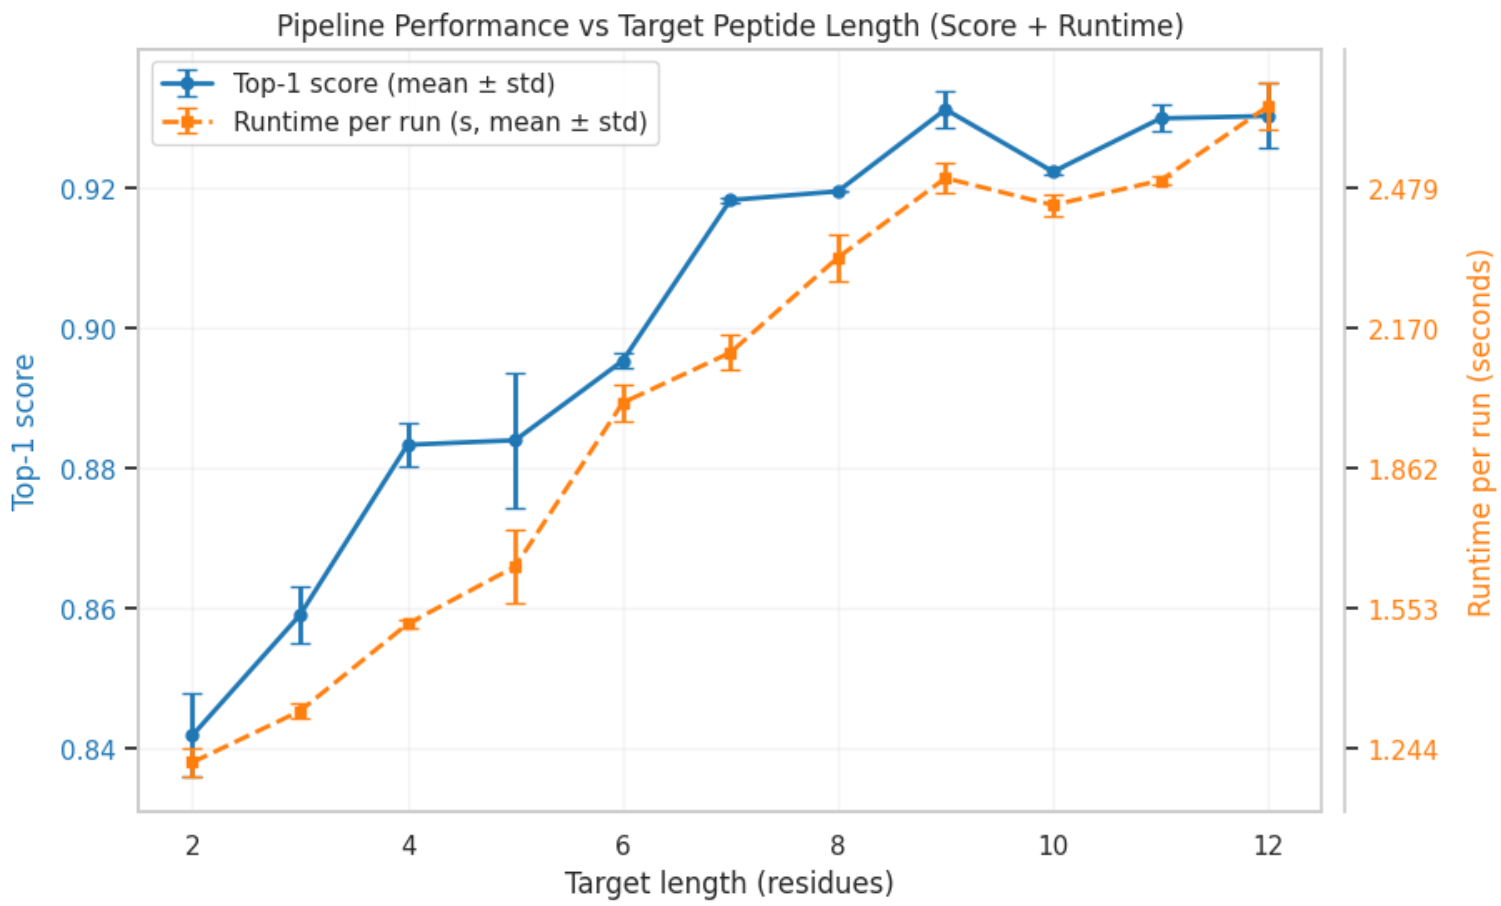
\includegraphics[width=\linewidth]{images/pipeline_performance_per_target_length.png}

        \column{0.36\textwidth}
        \begin{block}{Analyse}
            \footnotesize
            \begin{itemize}
                \item Les cibles très courtes (2--3) restent les plus difficiles.
                \item Le score remonte ensuite jusqu'à un plateau vers la longueur 11.
            \end{itemize}
        \end{block}
        
        \raggedleft \tiny \textcolor{gray}{Runtime: RTX 4070 (Portable), Ryzen 7350XT, 16Go RAM}
    \end{columns}
    \begin{alertblock}{Attention}
        \footnotesize
        Les scores élevés sur des longueurs pathologiques très courtes peuvent refléter
        une faiblesse de l'expert biologique plus qu'une plausibilité biologique réelle.
    \end{alertblock}


\end{frame}

\begin{frame}
    \frametitle{Pipeline vs baseline selon la difficulté}
    \begin{columns}[T,totalwidth=\textwidth]
        \column{0.58\textwidth}
        \centering
        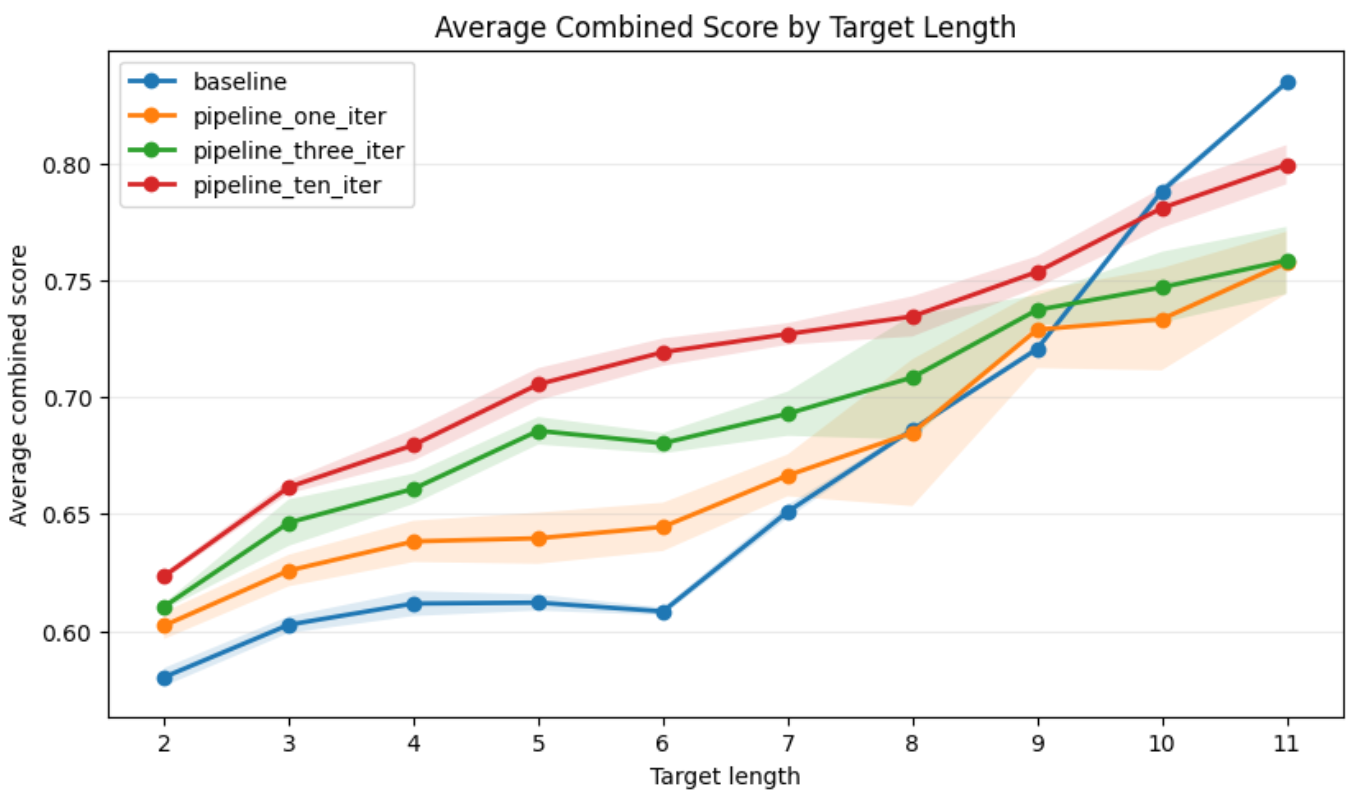
\includegraphics[width=\linewidth]{images/average_combined_score_by_target_length.png}

        \column{0.40\textwidth}
        \begin{block}{Analyse}
            \footnotesize
            \begin{itemize}
                \item Sur cibles courtes (difficiles), l'itération aide clairement
                \item Sur cibles longues (faciles), le gain n'est pas systématique
                \item Plus stable avec plus d'itérations
            \end{itemize}
        \end{block}

    \end{columns}
\end{frame}
